\question{Аксиально-симметричное электрическое поле. Распределение потенциала
  вблизи оси}

Во всех точках, находящихся на одинаковом расстоянии \( r \) от оси симметрии, 
поле должно быть одинаковым. При выборе в качестве системы координат 
цилиндрической системы \( (r, \phi, z ) \) с осью \( z \) совпадающей с осью 
симметрии, условие симметрии принимает вид \( \pder{}{\phi} = 0 \).

Для определения структуры электростатического поля воспользуемся уравнением 
Лапласа для потенциала:
\begin{equation}
	\D U = 0
	\label{eq08.2.9}
\end{equation}
где 
\( \D = \frac{1}{r}\pder{}{r}\left( r \pder{}{r} \right) + \ppder{}{z} \) -- 
оператор Лапласа в цилиндрической системе координат.

Решение этого уравнения будем искать в виде разложения в ряд по степеням 
\( r \): 
\begin{equation}
	U(r,z) = U_0 (z) + r^2 U_2 (z) + r^2 U_4 (z) + \ldots
	\label{eq08.2.10}
\end{equation}
причём чётность ряда по радиусу обусловлена именно аксиальной симметрией поля 
(см.рис.\ref{img08.1}), когда \( U(r,z) = U(-r,z) \).

\begin{figure}[h!]
	\center
	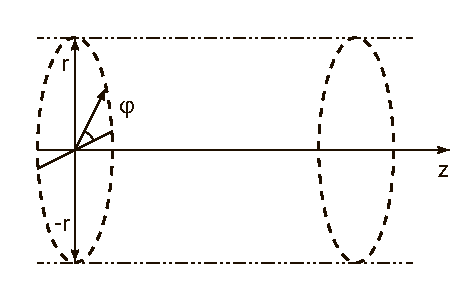
\includegraphics[width=.4\textwidth]{08_1}
	\caption{Схема осесимметричного электрического поля}
	\label{img08.1}
\end{figure}

Первый член \( U_0 (z) \) характеризует распределение потенциала вдоль оси 
симметрии (при \( r = 0 \)). Решение в виде (\ref{eq08.2.10}) имеет место, 
если оно удовлетворяет уравнению (\ref{eq08.2.9}). Для определения 
существования этого решения перепишем (\ref{eq08.2.9}) в виде
\begin{equation}
	\D U = \ppder{U}{z} + \frac{1}{r}\pder{U}{r} + \ppder{U}{r} = 0
	\label{eq08.2.11}
\end{equation}
и подставим в него соответствующие производные:
\[
	\begin{array}{c}
		\ppder{U}{z} = U_0''(z) + r^2 U_2''(z) + r^4 U_4''(z) + \ldots \\
		\frac{1}{r}\pder{U}{r} = 2U_2(z) + 4r^2U_4(z) + 6r^4U_6(z) + \ldots \\
		\ppder{U}{r} = 2U_2(z) + 12r^2U_4(z) + 30r^4U_6(z) + \ldots
	\end{array}
\]

Сгруппируем члены с одинаковыми степенями по \( r \):
\begin{equation}
	\left[ U_0''(z) + 4U_2(z) \right] + r^2\left[ U_2''(z) + 16U_4(z)\right] + 
		r^4\left[ U_4''(z) + 36U_6(z) \right] + \ldots = 0
	\label{eq08.2.12}
\end{equation}
Очевидно, что при любых \( r \) и \( z \) (\ref{eq08.2.12}) выполняются, если 
коэффициенты при \( r \) обращаются в нули. Получаем рекуррентные соотношения:
\begin{equation}
	\left. \begin{array}{c}
		U_2(z) = -\frac{1}{4}U_0^{(2)} = \frac{(-1)^1 U_0^{(2)}(z)}{2^2\cdot1} \\
		U_4(z) = -\frac{1}{64}U_0^{(4)} = 
			\frac{(-1)^2 U_0^{(2\cdot2)}(z)}{2^{2\cdot2}(1\cdot2)^2} \\
		U_6(z) = -\frac{1}{36\cdot64}U_0^{(4)}(z) = 
			\frac{(-1)^3 U_0^{2\cdot3}(z)}{(2\cdot3)(1\cdot2\cdot3)^2} \\
		\ldots \\
		U_{2n}(z) = (-1)^2\frac{U_0^{(2n)}(z)}{2^{2n}\cdot(n!)^2} \\
	\end{array} \right\}
	\label{eq08.2.13}
\end{equation}

Подставляя (\ref{eq08.2.13}) в (\ref{eq08.2.11}), находим выражение для 
распределения потенциала в любой точке: 
\[
	U(r,z) = U_0(z) - r^2 \frac{U_0^{(2)}}{4} + r^4 \frac{U_0^{(4)}}{64} - 
		\ldots,
\]
или, пользуясь тем, что \( 0! = 1 \) и \( 1! = 1 \), 
\begin{equation}
	U(r,z) = \sum\limits_{n=0}^{\infty}\frac{(-1)^2U_0^{(2n)}(z)}{(n!)^2}
		\left( \frac{r}{2} \right)^{2n}
	\label{eq08.2.14}
\end{equation}

Соотношение (\ref{eq08.2.14}) позволяет рассчитывать осесимметричные поля, 
если известно распределение потенциала на оси системы \( U_0(z) \).

Рассмотрим поле вблизи оси при малых \( r \) (в параксиальной области). 
Пренебрегая членами с порядка малости \( r^4 \) и выше, получаем:
\begin{equation}
	U(r,z) = U_0(z) - \frac{r^2}{4}U_0''(z)
	\label{eq08.2.15}
\end{equation}

Разложим \( U_0(z) \) в ряд Тейлора вблизи некоторой точки \( z_0 \):
\[
	U_0(z) = U_0(z_0) + U_0'(z_0)\D z + \frac{1}{2}U_0''(z_0)(\D z)^2 + \ldots
\]
Тогда распределение потенциала вблизи оси определяется соотношением
\begin{equation}
	U(r,z) = U_0(z_0) + U_0'(z_0)\D z + \frac{(\D z)^2}{2} U_0''(z_0) - 
		\frac{r^2}{4}U_0''(z)
	\label{eq08.2.16}
\end{equation}